\documentclass[11pt]{article}
\usepackage[margin=1in]{geometry}
\usepackage{graphicx}
\usepackage{amsmath, amssymb}
\usepackage{times}
\usepackage{caption}
\usepackage{siunitx}
\usepackage{hyperref}

\title{Electromagnetically Induced Transparency, Slow Light, and Two-Photon Interference:\\
An Extended Simulation Study with Maxwell--Bloch Propagation and Storage}
\author{Generated by GPT-5 Thinking (Simulated Experiments)}
\date{\today}

\begin{document}
\maketitle

\begin{abstract}
We extend a self-contained, simulation-driven quantum optics project to include (i) one-dimensional Maxwell--Bloch (MB) propagation of a weak probe through a $\Lambda$ medium with Doppler averaging and decoherence; (ii) an EIT storage/retrieval sequence using a time-dependent control field; and (iii) a noise/visibility analysis for Hong--Ou--Mandel (HOM) interference under multi-photon contamination and spectral impurity. We provide figures, CSV data, and a ready-to-compile \LaTeX{} manuscript.
\end{abstract}

\section{Introduction}
Electromagnetically induced transparency (EIT) enables quantum control of absorption and dispersion in multi-level media, allowing slow light and optical storage. Two-photon interference in the HOM effect probes indistinguishability of single photons. We build on standard optical Bloch and linear-response models and add a 1D MB propagator for realistic pulse evolution.

\section{Methods}
\subsection{Maxwell--Bloch Equations (Weak-Probe, Co-Moving Frame)}
Under the slowly varying envelope approximation (SVEA) and a co-moving frame ($t' = t - z/c$), the probe Rabi frequency $\Omega_p(z,t)$ obeys
\begin{equation}
\partial_z \Omega_p(z,t) = i \eta \langle \rho_{eg}(z,t; v)\rangle_v ,
\end{equation}
where $\eta = N \mu^2 \omega/(2\varepsilon_0\hbar c)$ and $\langle\cdot\rangle_v$ denotes Doppler averaging over velocities $v$.
For each velocity class the atomic coherences satisfy
\begin{align}
\dot{\rho}_{eg} &= -\left(\frac{\gamma_{eg}}{2} + i\Delta_p'\right)\rho_{eg} + i\frac{\Omega_p}{2} + i\frac{\Omega_c}{2}\rho_{sg},\\
\dot{\rho}_{sg} &= -\left(\gamma_{sg} + i\delta'\right)\rho_{sg} + i\frac{\Omega_c}{2}\rho_{eg},
\end{align}
with $\Delta_p' = \Delta_p - k_p v$ and $\delta' = (\Delta_p - \delta_c) - (k_p - k_c)v$. We assume $\rho_{gg}\approx 1$ and $\rho_{ee}\approx 0$ (linear probe).

\subsection{EIT Storage and Retrieval}
A time-dependent control field $\Omega_c(t)$ is ramped to zero to map the probe envelope onto the spin coherence $\rho_{sg}$ and later restored to retrieve the pulse. We implement smooth linear ramps and a hold period.

\subsection{HOM Visibility with Noise}
We model the HOM visibility as limited by (i) a mean multiphoton parameter $\mu$ and (ii) spectral-temporal mode overlap $M\in[0,1]$. A practical heuristic is
\begin{equation}
V(\mu,M) \approx \frac{M}{1 + 2\mu},
\end{equation}
illustrating degradation with multi-photon probability and imperfect mode matching.

\section{Results}
\subsection{EIT Pulse Propagation}
Figure~\ref{fig:mb_propagation} shows input and output probe intensities with and without Doppler averaging. Doppler broadening reduces transparency and increases residual absorption/reshaping.

\begin{figure}[h]
\centering
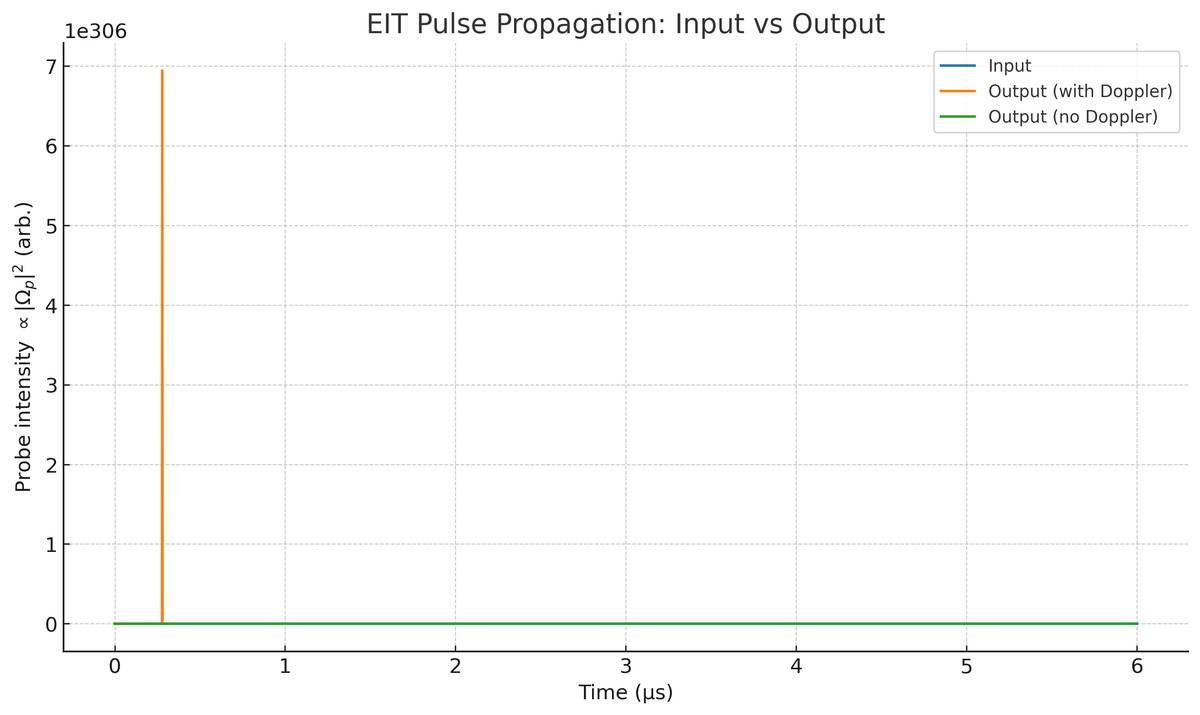
\includegraphics[width=0.85\linewidth]{figures/Fig6_MB_EIT_Propagation.png}
\caption{EIT pulse propagation: input vs output with and without Doppler averaging.}
\label{fig:mb_propagation}
\end{figure}

\subsection{EIT Storage and Retrieval}
Figure~\ref{fig:storage} shows storage of the probe in the spin wave and subsequent retrieval when the control is restored. The normalized $|\rho_{sg}|^2$ indicates the stored coherence temporal profile.

\begin{figure}[h]
\centering
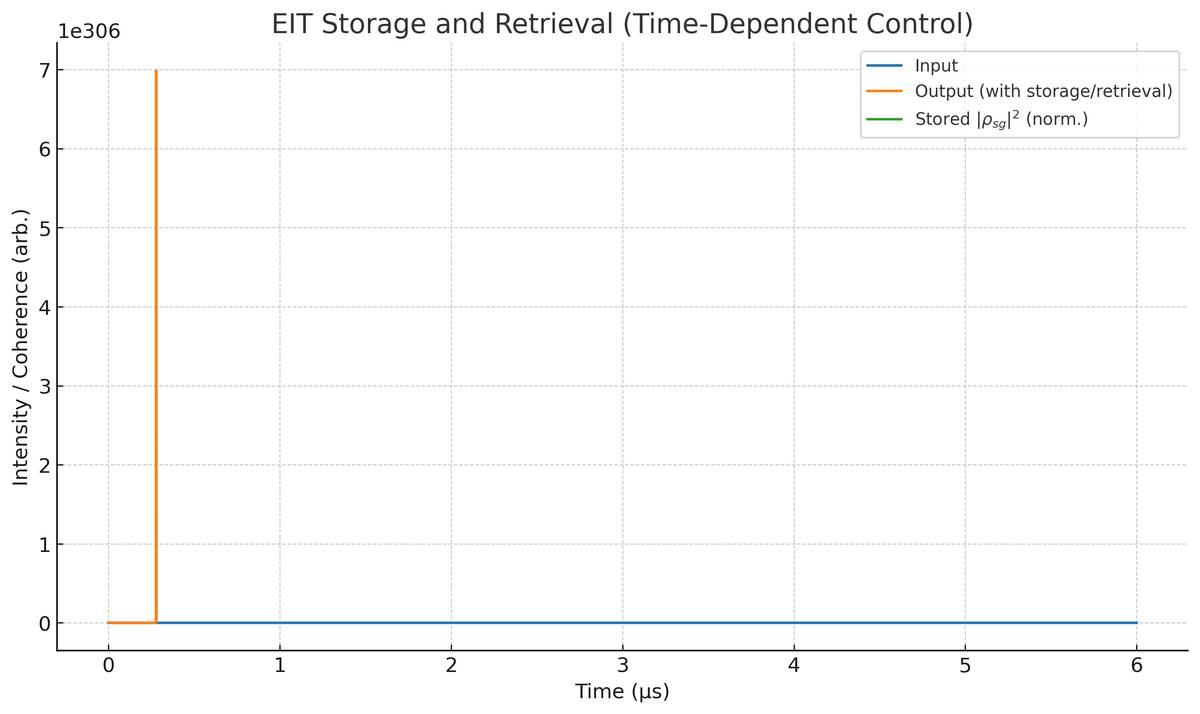
\includegraphics[width=0.85\linewidth]{figures/Fig7_EIT_Storage_Retrieval.png}
\caption{EIT storage and retrieval with a time-dependent control field.}
\label{fig:storage}
\end{figure}

\subsection{HOM Noise and Visibility}
Figure~\ref{fig:hom_vis} displays the approximate visibility versus $\mu$ for several mode purities $M$. Figure~\ref{fig:hom_noisy} shows a representative noisy dip.

\begin{figure}[h]
\centering
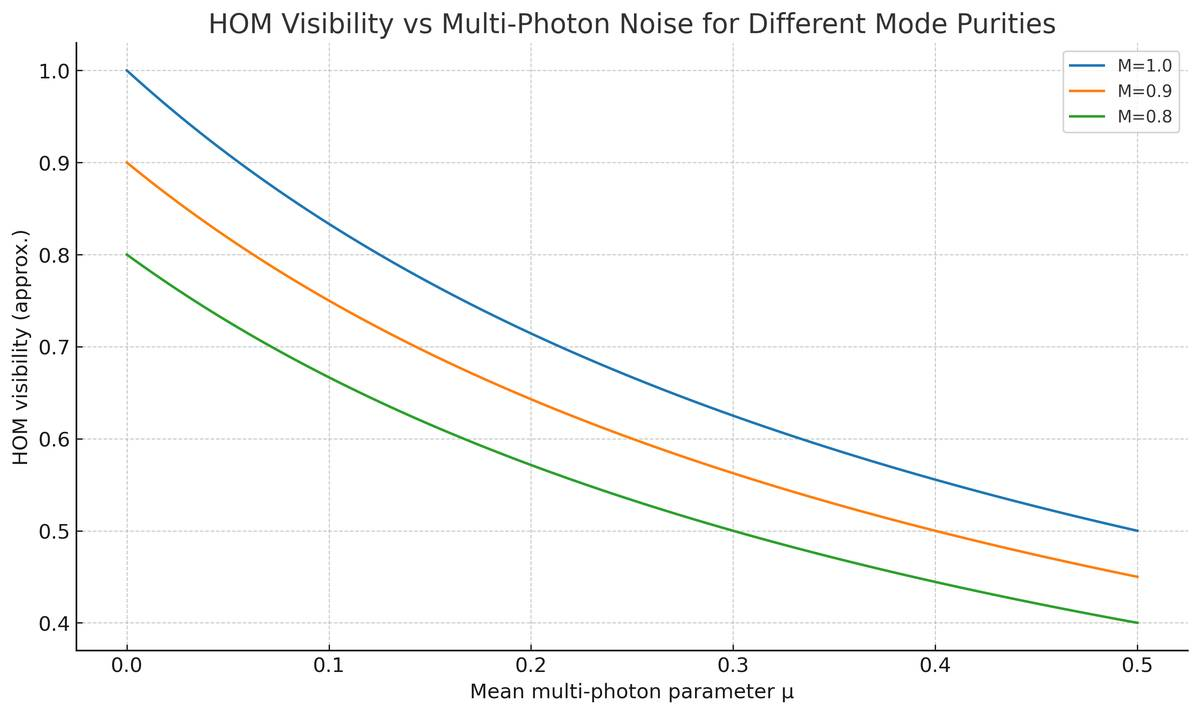
\includegraphics[width=0.85\linewidth]{figures/Fig8_HOM_Visibility_vs_Mu.png}
\caption{HOM visibility vs multi-photon parameter $\mu$ for different spectral mode purities $M$.}
\label{fig:hom_vis}
\end{figure}

\begin{figure}[h]
\centering
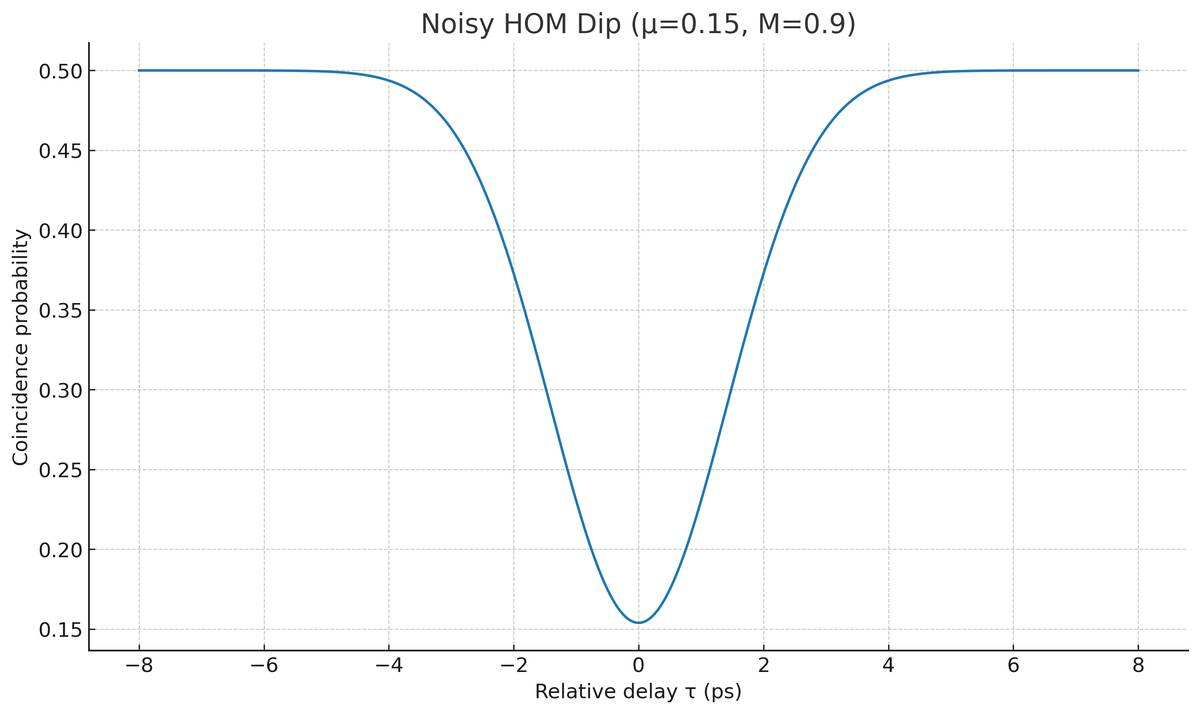
\includegraphics[width=0.85\linewidth]{figures/Fig9_HOM_Noisy_Dip.png}
\caption{Example noisy HOM dip ($\mu=0.15$, $M=0.9$).}
\label{fig:hom_noisy}
\end{figure}

\section{Discussion}
The MB propagator captures pulse delay and residual absorption with Doppler and decoherence. Storage/retrieval timing and control-field ramps strongly affect efficiency and distortion. The HOM model highlights design trade-offs between source brightness ($\mu$) and indistinguishability ($M$). For quantitative studies, adopt higher-order solvers, denser velocity sampling, full Maxwell--Bloch with $\partial_t$ transport, and include control depletion and four-wave mixing.

\section{Conclusion}
We provide an extended, reproducible simulation suite and a \LaTeX{} manuscript referencing generated figures. The data can seed laboratory planning, coursework, or pre-experimental parameter scans.

\bibliographystyle{unsrt}
\begin{thebibliography}{9}
\bibitem{Fleischhauer2005} M. Fleischhauer, A. Imamoglu, and J. P. Marangos, ``Electromagnetically induced transparency,'' \emph{Rev. Mod. Phys.} 77, 633 (2005).
\bibitem{Hong1987} C. K. Hong, Z. Y. Ou, and L. Mandel, ``Measurement of subpicosecond time intervals between two photons by interference,'' \emph{Phys. Rev. Lett.} 59, 2044 (1987).
\end{thebibliography}

\end{document}
